% ++++++++++++++++++++++++++++++++++++++++
% Don't modify this section unless you know what you're doing!
\documentclass[letterpaper,12pt]{article}
\usepackage{tabularx} % extra features for tabular environment
\usepackage{amsmath}  % improve math presentation
\usepackage{graphicx} % takes care of graphic including machinery
\usepackage[margin=0.75in,letterpaper]{geometry} % decreases margins
\usepackage{cite} % takes care of citations
\usepackage[final]{hyperref} % adds hyper links inside the generated pdf file
\usepackage{listings}
\usepackage{csvsimple}
\usepackage{verbatim}
\usepackage{float}
\usepackage{graphicx} % Allows including images
\hypersetup{
	colorlinks=true,       % false: boxed links; true: colored links
	linkcolor=black,        % color of internal links
	citecolor=blue,        % color of links to bibliography
	filecolor=magenta,     % color of file links
	urlcolor=blue         
}
%++++++++++++++++++++++++++++++++++++++++
\setlength{\parindent}{0pt}
\setlength\parskip{1em plus 0.1em minus 0.2em}

\begin{document}
\title{%
Instruments and Wiring \\ \\
\large The Output Resistance of a Power Supply\\
\large PHY224 Lab 5}
\author{Fredrik Dahl Bråten, Pankaj Patil}
\date{\today}
\maketitle
%\tableofcontents
%\listoffigures
%\listoftables

\section{Abstract}

In this exercise, we measure and model the current and voltage of two circuit diagrams, 
first with a battery, and then later with a power supply. As the only difference between 
the diagrams is the placement of the ammeter and the voltmeter, we can with these two setups determine 
the resistance of the ammeter, the current through the voltmeter, and the internal 
resistance of the battery. All these three parameters are usually assumed to be negligible. 
We will use a linear function to model the relation between the total voltage and the total 
current through the circuit. To evaluate the quality of our models, we calculate and discuss 
the $\chi_{red}^2$ value of our model and data. This analysis was done in Python by use of the numpy, scipy and matplotlib modules.

\section{Introduction}

In this exercise, we measure and model the current and voltage of two circuit diagrams, 
first with a battery and then later with a power supply, see OutputResist.pdf. 
The theoretically predicted relationship between the terminal voltage ($V_1$), the open circuit voltage 
($V_{\infty}$), the current passing between the nodes of the battery/power supply ($I_2$) 
and the output resistance of the power source ($R_{internal}$), is:
$$V_1 = V_{\infty} – R_{internal}I_2$$
This relationship is modeled by a linear relationship $y = ax+b$.
Furthermore, we know that the terminal voltage $V_{PS} = V_1$, the voltage measured 
in the circuit configuration 1. The voltage difference over the resistor $V_R = V_2$, 
the voltage measured in the circuit configuration 2. Also, the potential difference over the ammeter $V_A = V_{PS} – V_R$.
By this notation, we also have the following relations: 

$I_{PS} = I_2, I_R = I_1, I_V = I_{PS} – I_R$, and thus 

$I_V = I_2 - I_1.$

Furthermore, by Ohms law, we have 
$R_A = V_A / I_A = V_{A1} / I_{A1} = (V_{PS} – V_R)/I_1 = (V_1 – V_2)/ I_1.$

Thus, we have the relations for the current through the voltmeter, $I_V = I_2 – I_1$, 
and the relation for what resistance the ammeter has: $R_A =  (V_1 – V_2)/ I_1$.

In our experiment, $V_1$ and $V_2$ are our dependent variables, while $R_{internal}$, $R_A$, $I_1$, and $I_2$, are independent variables.

\section{Methods, Materials and Experimental Procedure}

We successfully followed the procedures as described in the OutputResist.pdf document.

\section{Results}

From our model of the total voltage and current, for the 6V battery, we found that:

$V_{\infty} = 6.31 \pm 0.1\ V$

$R_{internal} = 0.77 \pm 2.209\ Ohm$ (using the standard deviation of the power supply internal resistance estimates as uncertainty).

$\chi_{red}^2 = 0.00020972$

Similarly, for our power supply with the 6V setting:

$V_{\infty} = 6.00 \pm 0.1\ V$

$R_{internal} = 48.37 \pm 2.209\ Ohm$

$\chi_{red}^2 = 0.00006698$

For the power supply with the 10V setting:

$V_{\infty} = 10.00 \pm 0.1\ V$

$R_{internal} = 51.73 \pm 2.209\ Ohm$

$\chi_{red}^2 = 0.00000218$

For the power supply with the 15V setting:

$V_{\infty} = 15.00 \pm 0.1\ V$

$R_{internal} = 45.84 \pm 2.209\ Ohm$

$\chi_{red}^2 = 0.00002729$

For the power supply with the 20V setting:

$V_{\infty} = 20.00 \pm 0.1\ V$

$R_{internal} = 46.99 \pm 2.209\ Ohm$

$\chi_{red}^2 = 0.00000242$

Therefore, the average internal resistance of the power supply with uncertainty, 
estimated from these measurements are:
$R_{internal\ (power\ supply)} = 48.23 \pm 1.1045\ Ohm$ (uncertainty = $2.209/\sqrt{N}$).
We will associate a similar uncertainty to our estimate of the battery’s internal resistance, as that experiment were performed similarly to those with the power supply:
$R_{internal\ (battery)} = 0.77 \pm 1.88\ Ohm$.
This will be our estimate of the internal resistance of the power supply and battery.

Furthermore, averaging and taking the standard deviation of each ammeter resistance
 estimate from the 6 resistors for the 4 different voltage settings of the power 
 supply, we find that our estimate of the resistance of the ammeter is: 16.9 $\pm$ 7.18 Ohm
The voltage passing through the voltmeter varies for each voltage setting, but for 
instance, the current through the voltmeter is: -0.00012 Ampere when the total current through the 
circuit is 0.0059 Ampere, the terminal voltage is: 6 volts, and the resistor in the circuit is 100.0 kilo Ohm.
Run the python script in the appendix to get all the different currents through the voltmeter for each resistor and power supply setting.

Below in Figure [1]-[5], we see our data from the experiments plotted as points with corresponding error bars. Furthermore, we see the curve of our model fitted to the data, as described in the introduction. 

\begin{figure}[H]
  \centering
  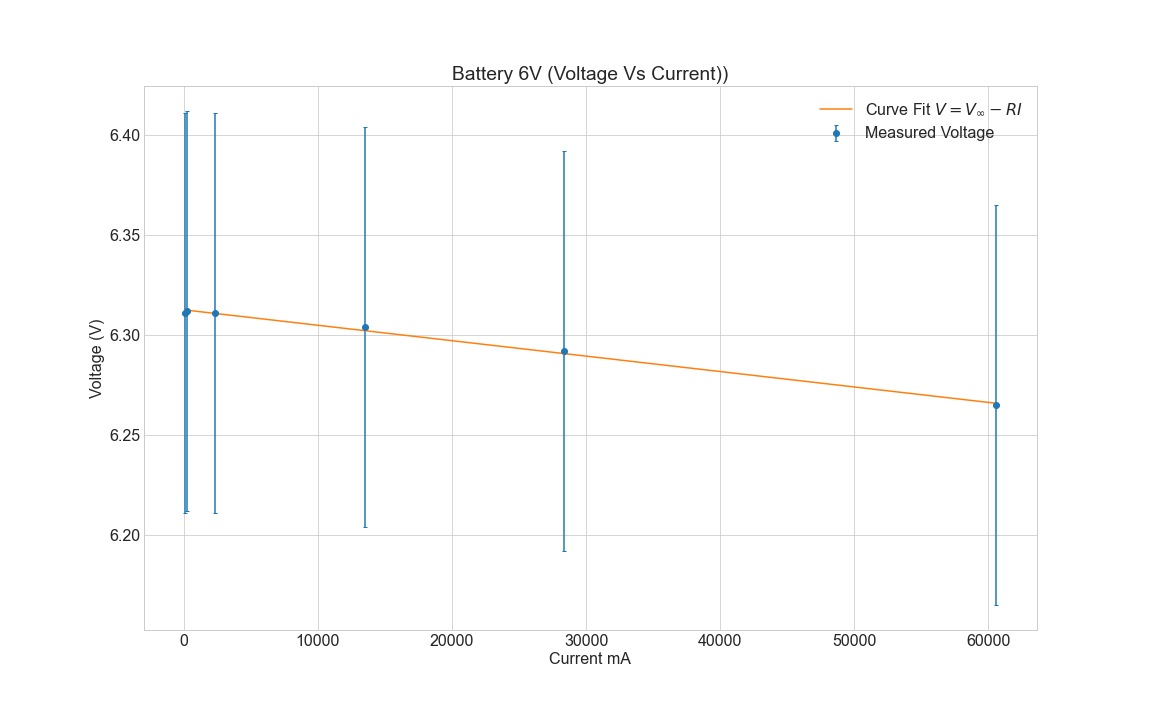
\includegraphics[width=0.95\linewidth]{../code/Fredrik/6V battery lab5_voltage_vs_current.png}    
  \begin{center}
    \begin{center}
      Model Function : $V = V_{\infty} - RI$ \\
      $V_{\infty} = 6.31 \pm 0.05 $ V\\
      $R = 0.77 \pm 1.88$ Ohm\\
    \end{center}  \end{center}
  \caption{6V Battery: Voltage vs. Current}
  \label{battery-v-i}
\end{figure}

\begin{figure}[H]
  \centering
  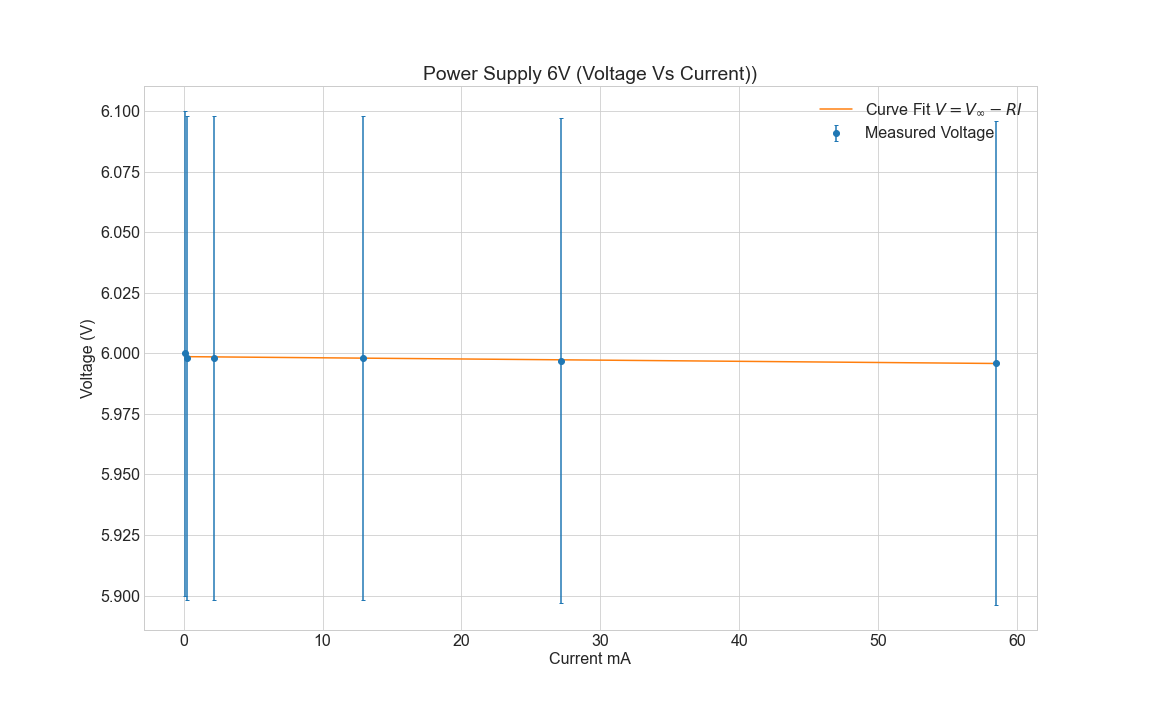
\includegraphics[width=0.95\linewidth]{../code/Fredrik/Power supply 6V lab5_voltage_vs_current.png}    
  \caption{Power Supply 6V (Voltage vs Current)}
  \label{ps-6}
\end{figure}

\begin{figure}[H]
  \centering
  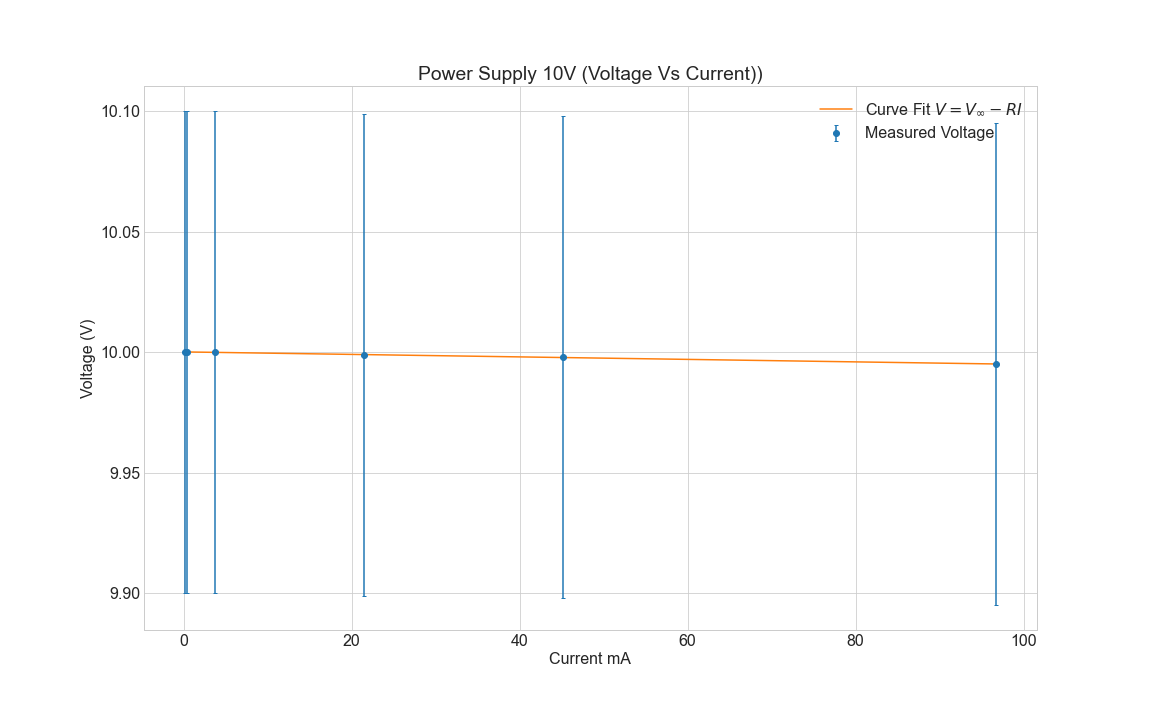
\includegraphics[width=0.95\linewidth]{../code/Fredrik/Power supply 10V lab5_voltage_vs_current.png}    
  \caption{Power Supply 10V (Voltage vs Current)}
  \label{ps-10}
\end{figure}

\begin{figure}[H]
  \centering
  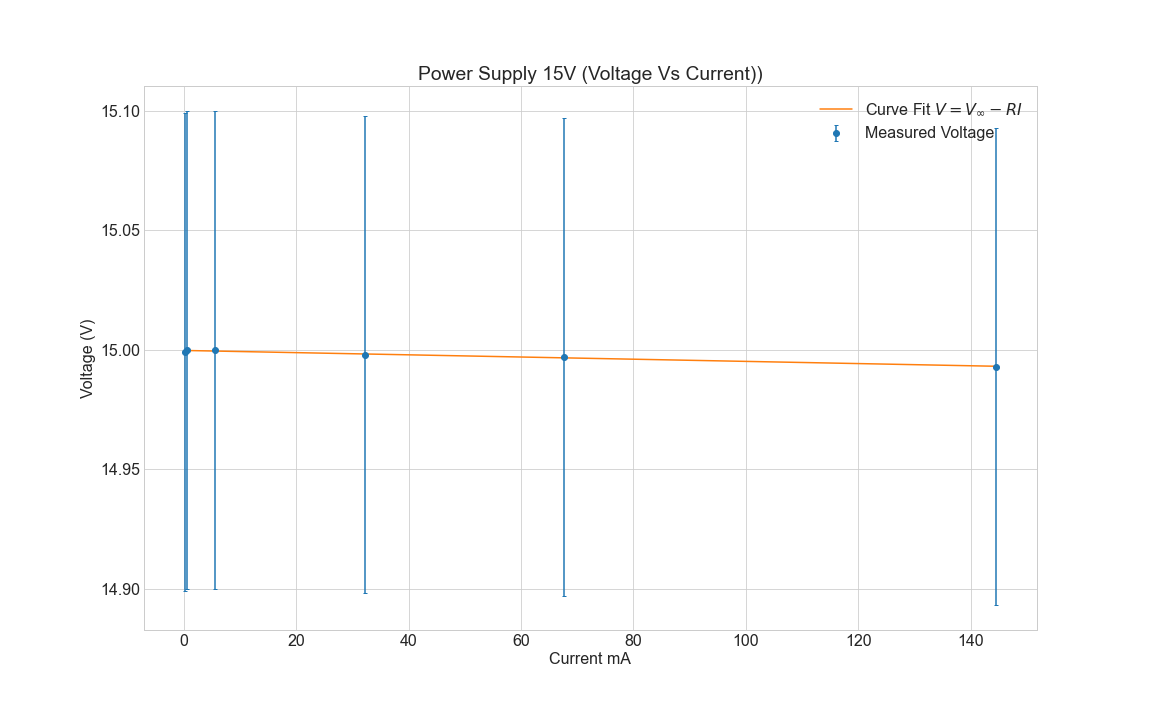
\includegraphics[width=0.95\linewidth]{../code/Fredrik/Power supply 15V lab5_voltage_vs_current.png}    
  \caption{Power Supply 15V (Voltage vs Current)}
  \label{ps-15}
\end{figure}

\begin{figure}[H]
  \centering
  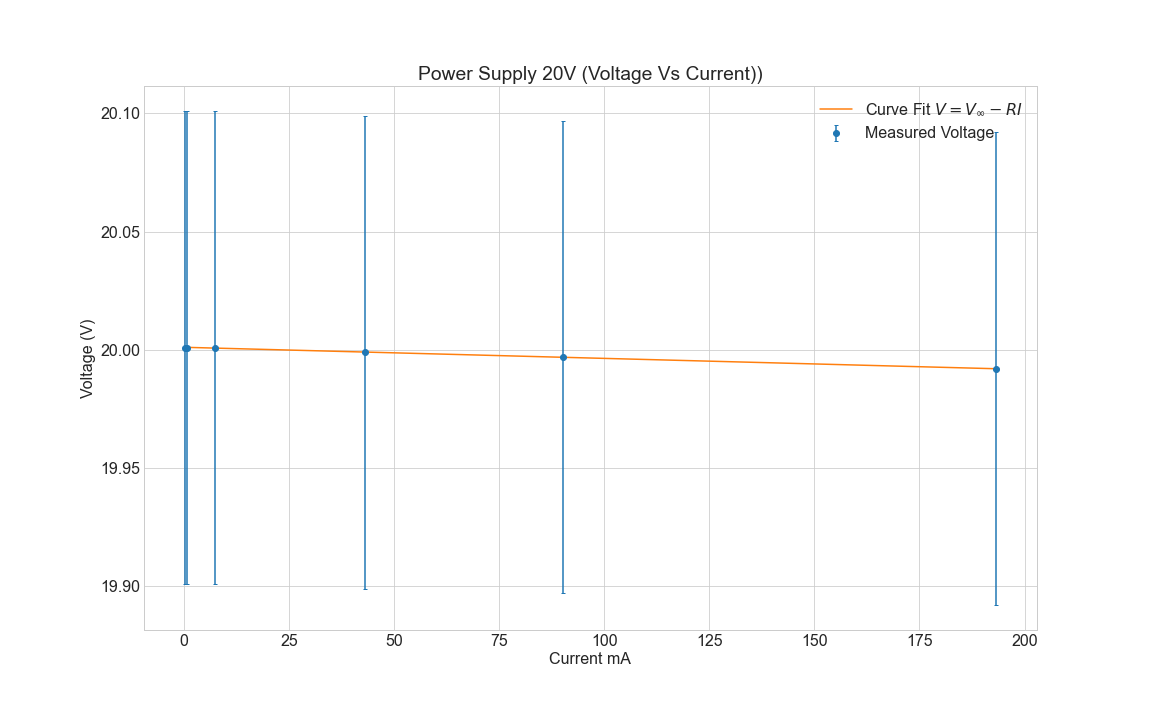
\includegraphics[width=0.95\linewidth]{../code/Fredrik/Power supply 20V lab5_voltage_vs_current.png}    
  \caption{Power Supply 20V (Voltage vs Current)}
  \label{ps-20}
\end{figure}

\begin{figure}[H]
  \centering
  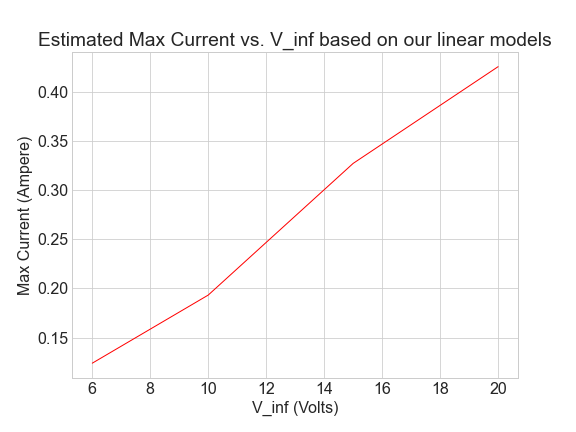
\includegraphics[width=0.95\linewidth]{../code/Fredrik/Estimated Max Current vs. V_inf based on our linear models.png}    
  \caption{6V Battery: Maximum Current vs. $V_{\infty}$ }
  \label{ps-max-c}
\end{figure}

\section{Discussion}

The $\chi_{red}^2$ values we found were very low. This means that our models fit our data very well. 
However, our $\chi_{red}^2$ values should ideally be equal to one for most experiments. 
That we have extremely low $\chi_{red}^2$ values implies that we do not have enough data. 
It means that we are in risk of overfitting our models to our data. However, 
this exercise asked for data from four resistors, while we used six. 
Thus, in our case, the small $\chi_{red}^2$ values is a good sign, as it means that 
we have good linear data for which our model fits nicely. Furthermore,
 both models are well within the uncertainties of our measurements, 
 see Figure [1] to [5] in the Results section.
As we can see from the current passing through the voltmeter, 
it is very small in comparison to the measured total current in the circuit, see the results section. 
This is a good sign, as ideally no current should pass through the voltmeter. 
The current is also negative, which is not a surprising result. 
Within the voltmeter there is a battery made for compensating for the drop in voltage 
caused by the presence of the voltmeter in the circuit. If this battery overcompensates 
for the voltage drop, current will flow in the opposite direction of normal 
flow (according to the power supply). This is what we observe.
Furthermore, the estimated resistance of the ammeter is small in comparison to the 
resistance of the different resistors for which we used in our circuits. 
Whether the resistance is negligible depends on the resistance of the resistor 
in the circuit, which in our experiments varied in size from 100Ohm to 100k Ohm.
The estimated internal resistance of the power supply was large and significant 
in comparison to the smaller resistors we used, though negligible for the larger 
resistors we used. We got satisfactory small uncertainties in our estimate of the 
internal resistance for the power supply. However, for the battery, the estimated 
internal resistance was indeed very small and negligible in comparison to all the 
resistors in our experiments.
Now for answering the specific questions in the lab manual:

\textbf{Question 1}

There is no better circuit diagram of the two. In the first one, 
the voltmeter measures the total potential difference in the circuit over the battery, 
while the ammeter measures the current flowing through the resistor. 
In the second diagram, the voltmeter measures the voltage difference over the resistor, 
while the ammeter measures the total current flowing in the circuit, 
from one node to the other of the battery. Together, measurements of current 
and voltage for each of the diagrams, determine what current run through the resistor, 
what current run through the voltmeter, and what current runs from the cathode 
to the anode of the battery. Likewise, we are able to determine the potential 
difference over the battery, over the resistor, and over the ammeter. 
With ideal multimeters, there should however be no difference between the two.

\textbf{Question 2}

We chose to measure current and voltage for the two diagrams with as 
many different resistors as possible, of those we had easily available, to 
increase our $\chi_{red}^2$ value for our model. Thus, we used all six resistors 
on the circuit board. Furthermore, statistically by the central limit theorem, 
a higher number of measurements results in a lower uncertainty in our estimates 
for the internal resistances of the battery, power supply and ammeter along with 
the current through the voltmeter, when averaging.

\textbf{Question 3}

See introduction. Furthermore, though $I_V$ varies for each resistor and power 
supply voltage, by averaging the estimated $R_A$ for the data associated with 
each resistor and power supply/battery voltage, we can get a better estimate of $R_A$, 
see the results section.

As we mentioned previously in the discussion, the resistance of the ammeter is 
small and negative. This is due to its large resistance and the overcompensation 
for voltage by the small internal battery of the voltmeter.

\textbf{Question 4}

See plots in the Results section to see the estimated relationship between 
the current and voltage of the circuit according to our data. For the range 
of resistors for which we utilized in our experiments with the power supply, 
the current and voltage followed a linear relationship. However, according to 
the theory, for higher currents, we should see a non-linear relationship. 
However, we never reached currents which formed non-linear relationships with the voltage. 

However, the maximum current is the current between the terminals of the power supply when 
$V_{\infty}$ is approaching zero. We can estimate this value from our linear relations, 
though this will be a poor fit with the theoretically predicted maximum current, 
if the voltage current-relationship is non-linear at higher currents:
At $I_{max}$, V=0, thus according to the equation from the introduction, $V = V_{\infty} – R_{internal}I$
So, $I_{max} = V_{\infty}/R_{internal}$.
We then get an increasing relationship between $V_{\infty}$ and $I_{max}$, see Figure [6] in 
the Results section.


\section{Conclusions}

In this exercise, we measure and model the current and voltage of two circuit diagrams, 
first with a battery, and then later with a power supply. We successfully followed the 
instructions for the experiments written in the OutputResist.pdf lab manual. We have plotted 
our data with error bars, along with our corresponding linear models. Furthermore, 
we have calculated and discussed the $\chi_{red}^2$ values of the models, and estimated 
the internal resistance of the power supply, the battery, the ammeter, and the current 
flowing through the voltmeter. Finally, we have answered the questions of the lab manual. 

\pagebreak

\appendix

\section{Appendix}

\subsection{Python Code: Battery 6V}

The Python code for this exercise is divided into two files. statslab.py file contains utility methods
which we will be frequently using in this course. lab\_5\_battery.py file contains the code which analyzes
the data.

\subsubsection{statslab.py}
\noindent\rule{\textwidth}{1pt}
\verbatiminput{../code/Pankaj/statslab.py}
\noindent\rule{\textwidth}{1pt}

\pagebreak

\subsubsection{lab\_5\_battery.py}
\noindent\rule{\textwidth}{1pt}
\verbatiminput{../code/Pankaj/lab_5_battery.py}
\noindent\rule{\textwidth}{1pt}

\pagebreak

\subsection{Python Code: Power Supply}

The Python code for this exercise is divided into four files. statslab.py in included in previous section. Code 1.py and Code 2.py
analyze the data for Power Supply

\subsubsection{Functions.py}
\noindent\rule{\textwidth}{1pt}
\verbatiminput{../code/Fredrik/Functions.py}
\noindent\rule{\textwidth}{1pt}

\pagebreak

\subsubsection{Code 1.py}
\noindent\rule{\textwidth}{1pt}
\verbatiminput{../code/Fredrik/Code 1.py}
\noindent\rule{\textwidth}{1pt}

\pagebreak

\subsubsection{Code 2.py}
\noindent\rule{\textwidth}{1pt}
\verbatiminput{../code/Fredrik/Code 2.py}
\noindent\rule{\textwidth}{1pt}

\pagebreak

\begin{thebibliography}{99}

\bibitem{lab-manual-ex5} Lab Manual - OutputResist.pdf

\end{thebibliography}

\end{document}
